\chapter{连续介质力学} \label{chap2}
\section{引言}
连续介质力学是本文构建控制方程的理论基础。
基于连续介质力学,我们刻画流体以及流体表面,并从两个
视角来描述物体运动,以此构建动力学方程。为了构建完整的控制方程,我们还需要给出本构模型,
即形变与势能的关系,这里我们给出对应的流体的弱可压缩模型以及表面张力模型。

\section{欧拉视角下的动力学}
欧拉视角,即物理量的定义域为$\mathbb{R}^3$,对物体的刻画由空间中的密度场给出。与拉格朗日视角的区别我们将在2.3小节中给出。

\subsection{欧拉视角下的质量守恒定律}
记$\rho : \mathbb{R}^3 \times \mathbb{R} \rightarrow \mathbb{R}$ 为空间中随时间变化的密度场,
$v : \mathbb{R}^3 \times \mathbb{R} \rightarrow \mathbb{R}^3$ 为空间中随时间变化的速度场。
\begin{figure}[htbp]
    \centering
    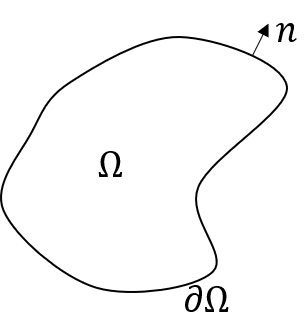
\includegraphics[scale=0.5]{./images/image1.png}
    \caption{}
    \label{fig:example}
\end{figure}

现在考虑一个$\mathbb{R}^3$闭区域$\Omega$,$\Omega$的边界记为$\partial \Omega$,边界上的法向记为
$n$(如图2.1)。同时假定$\rho$ 和 $v$在 $\Omega \times (t_0 - \epsilon, t_0 + \epsilon)$的一个开邻域内足够光滑。根据质量守恒,我们有$\Omega$上质量的
变化率为$\partial \Omega$上质量的流出率和流入率之和。即
\begin{equation}
    \begin{split}
        \frac{d}{dt} \Big |_{t = t_0}\int_{\Omega} \rho(x,t)dx &= -\int_{\partial \Omega} \rho(x,t_0) v(x,t_0) \cdot n(x) ds \\
        \int_{\Omega} \frac{\partial}{\partial t}\Big |_{t = t_0} \rho (x,t)dx &= -\int_{\partial \Omega} div(\rho(x,t_0) v(x,t_0))dx\nonumber\\
    \end{split}
\end{equation}

由于$\Omega$的任意性,由上式可以得到

\begin{equation}
    \frac{\partial}{\partial t}\Big |_{t = t_0}\rho(x,t) + div(\rho v) = 0
\end{equation}

\subsection{欧拉视角下的动量守恒定律}
现在考虑闭区域$\Omega$上的动量变化,根据连续介质力学中的牛顿运动定律,




\section{拉格朗日视角下的动力学}
\section{弱可压缩流体}
\section{表面张力}

